\subsection*{Modelli 5 - \textit{size}-ukra-0}

% Introduzione su strategia del training -> qual è l'obiettivo dell'esperimento?

Per replicare i risultati si è deciso di essere il puù fedeli possibili con gli iperparametri 
noti e a disposizione nell'articolo dei ricercatori ucraini e di testare le 3 dimensioni di modelli
di YOLO che fino a quel momento sono stati sfruttati: nano (YOLOv8n), small (YOLOv8s) e medium (YOLOv8m).
Pertanto i nomi dei modelli addestrati fanno riferimento come \textit{size}\texttt{-ukra-0} per 
evidenziare come questi modelli siano svolti prendendo in riferimento le configurazioni degli 
esperimenti degli autori dell'articolo.

Le fasi di addestramento sono stati svolti non più su server colab ma sui server interni 
all'università dove venivano messi a disposizione 2 GPU T4. Il motivo principale dell'utilizzo dei 
server era dovuto non tanto a questo esperimento ma a quello successivo comprendente una fase di 
tuning che risultava particolarmente onerosa.

Gli iperparametri, tabella \ref{tab:v5-model-configs}, sono stati impostati esattamente ai valori citati nell'articolo e impostati
ai valori di default qualora l'iperparametro non venisse menzionato. Il numero di epoche è stato inizialmente
impostato a 600 con il modello \texttt{small} e patience pari a 300. Avendo poi visionato i 
risultati si è deciso di ridurre il numero di epoche a 200 e la patience a 50 per le altre due 
dimensioni. Il modello \texttt{medium} ha poi subito un arresto verso la fine dell'addestramento. Non 
abbiamo pertanto i grafici dell'addestramento a disposizione ma solo le metriche ricavate dalla validazione
sul test set. 

% Dettagli configurazione, tipologia modello e iperparametri, dove è stato eseguito il train

\begin{table}[!htb]
    \centering
    \begin{tabular}{lccc}
        \hline
        \textbf{Iperparametro} & \textbf{nano} & \textbf{small} & \textbf{medium}\\
        \hline
        epoche & 200 & 600 & 200 \\
        optimizer & Adam & Adam & Adam\\
        learning rate (lr0) & 0.0001 & 0.0001 & 0.0001\\
        learning rate (lrf) & 0.01 & 0.01 & 0.01\\
        momentum & 0.98 & 0.98 & 0.98\\
        weight\_decay & 0.0005 & 0.0005 & 0.0005\\
        imgsz & 800 & 800 & 800\\
        dropout & 0.0 & 0.0 & 0.0 \\
        patience & 50 & 300 & 50\\
        \midrule
        hsv\_h & 0.4 & 0.4 & 0.4 \\
        degrees & 0.0 & 0.0 & 0.0  \\
        shear & 0.0 & 0.0 & 0.0 \\
        \hline
    \end{tabular}
    \caption{Configurazione iperparametri dei modelli \textit{size}\texttt{-ukra-0} per il training}
    \label{tab:v5-model-configs}
    \end{table}

    
    % Dettagli configurazione, tipologia modello e iperparametri, dove è stato eseguito il train

% Risultati training
% - andamento training


  %----------------------------

  \begin{figure}[!htb]
    \centering
    \includegraphics[width=0.8\textwidth]{v_5/small-ukra-0/results.png}
        \caption{Andamento funzioni di loss e metriche durante l'esecuzione di \texttt{small-ukra-0}}
        \label{fig:v5-2}
    \end{figure}
    % - grafici recall e precision e performance e F1
    \begin{figure}[!htb]
        \centering
        \begin{subfigure}{.5\textwidth}
            \centering
            \includegraphics[width=.9\linewidth]{v_5/small-ukra-0/P_curve.png}
            \subcaption{P-curve}
            \label{fig:v5-3.1}
        \end{subfigure}%
          \begin{subfigure}{.5\textwidth}
            \centering
            \includegraphics[width=.9\linewidth]{v_5/small-ukra-0/R_curve.png}
            \subcaption{PR-curve}
            \label{fig:v5-3.2}
        \end{subfigure}
        \vskip\baselineskip
        \begin{subfigure}{.5\textwidth}
            \centering
            \includegraphics[width=.9\linewidth]{v_5/small-ukra-0/PR_curve.png}
            \subcaption{PR-curve}
            \label{fig:v5-3.3}
        \end{subfigure}
        \begin{subfigure}{.49\textwidth}
            \centering
            \includegraphics[width=.9\linewidth]{v_5/small-ukra-0/F1_curve.png}
            \subcaption{F1-curve}
            \label{fig:v5-3.4}
        \end{subfigure}
        
        \caption{Andamento funzioni di loss e metriche durante l'esecuzione di \texttt{small-ukra-0}}
        \label{fig:v5-3}
    \end{figure}

% -------------------------
Come si può notare dalle figure \ref{fig:v5-2} e \ref{fig:v5-6}, l'andamento
delle funzioni di errore durante la fase di training scendono velocemente fino
a raggiungere valori molto al di sotto di quelli trovati finora. Ma se si 
guarda l'andamento delle funzioni di errore nelle fasi di validazione si può
vedere come l'errore risulta più simile ai precedenti tentativi rispetto ai risultati
mostrati nell'articolo. Anche le metriche raggiungono abbastanza velocemente una fase di 
saturazione delle prestazioni che però non sono soddisfacenti, ben al di sotto di 
quelle preannunciate.

\begin{figure}[!htb]
    \centering
    \includegraphics[width=0.8\textwidth]{v_5/nano-ukra-0/results.png}
        \caption{Andamento funzioni di loss e metriche durante l'esecuzione di \texttt{nano-ukra-0}}
        \label{fig:v5-6}
    \end{figure}
    % - grafici recall e precision e performance e F1
    \begin{figure}[!htb]
        \centering
        \begin{subfigure}{.5\textwidth}
            \centering
            \includegraphics[width=.9\linewidth]{v_5/nano-ukra-0/P_curve.png}
            \subcaption{P-curve}
            \label{fig:v5-5.1}
        \end{subfigure}%
          \begin{subfigure}{.5\textwidth}
            \centering
            \includegraphics[width=.9\linewidth]{v_5/nano-ukra-0/R_curve.png}
            \subcaption{PR-curve}
            \label{fig:v5-5.2}
        \end{subfigure}
        \vskip\baselineskip
        \begin{subfigure}{.5\textwidth}
            \centering
            \includegraphics[width=.9\linewidth]{v_5/nano-ukra-0/PR_curve.png}
            \subcaption{PR-curve}
            \label{fig:v5-5.3}
        \end{subfigure}
        \begin{subfigure}{.49\textwidth}
            \centering
            \includegraphics[width=.9\linewidth]{v_5/nano-ukra-0/F1_curve.png}
            \subcaption{F1-curve}
            \label{fig:v5-5.4}
        \end{subfigure}
        
        \caption{Andamento funzioni di loss e metriche durante l'esecuzione di \texttt{nano-ukra-0}}
        \label{fig:v5-5}
    \end{figure}
    
    Dalla tabella \ref{table:v5-1} possiamo vedere come il modello migliore sia quello
\texttt{small} ma questo non supera il valore di mAP del 34.9\%, al di sotto di alcuni
risultati raggiunti nei tentativi precedenti. Questa discrepanza di prestazioni tra 
i nostri valori e quelli indicati nell'articolo suggeriscono un qualche problema di fondo.

    \begin{table}[!htb]
        \centering
        \begin{tabularx}{\textwidth}{lYYYc}
            \toprule
            Class & P & R & mAP50 & mAP50-95 \\
            \midrule
            \texttt{small-ukra-0} \\
            \midrule
            ALL & 0.432 & 0.406 & 0.349 & 0.178 \\
            PLASTIC\_BAG & 0.304 & 0.329 & 0.201 & 0.0628 \\
            PLASTIC\_BOTTLE & 0.725 & 0.747 & 0.763 & 0.414 \\
            OTHER\_PLASTIC\_WASTE & 0.168 & 0.197 & 0.100 & 0.0309 \\
            NOT\_PLASTIC\_WASTE & 0.533 & 0.351 & 0.332 & 0.205 \\
            \midrule
            \texttt{nano-ukra-0} \\
            \midrule
            ALL & 0.330 & 0.379 & 0.308 & 0.149 \\
            PLASTIC\_BAG & 0.212 & 0.235 & 0.155 & 0.0506 \\
            PLASTIC\_BOTTLE & 0.695 & 0.737 & 0.744 & 0.372 \\
            OTHER\_PLASTIC\_WASTE & 0.143 & 0.254 & 0.104 & 0.0293 \\
            NOT\_PLASTIC\_WASTE & 0.271 & 0.288 & 0.229 & 0.144 \\
            \midrule
            \texttt{medium-ukra-0} \\
            \midrule
            ALL & 0.405 & 0.394 & 0.324 & 0.168 \\
            PLASTIC\_BAG & 0.209 & 0.235 & 0.124 & 0.0418 \\
            PLASTIC\_BOTTLE & 0.738 & 0.754 & 0.771 & 0.415 \\
            OTHER\_PLASTIC\_WASTE & 0.146 & 0.246 & 0.089 & 0.0280 \\
            NOT\_PLASTIC\_WASTE & 0.527 & 0.342 & 0.311 & 0.186 \\
            \bottomrule
        \end{tabularx}
        \caption{Risultati delle metriche sul test set per \textit{size}\texttt{-ukra-0}}
        \label{table:v5-1}
    \end{table}

Da una parte è plausibile un qualche nostro errore ma strano che porti a risultati
tanto disastrosi. Dall'altra parte è possibile che i risultati pubblicati dai 
ricercatori non siano affidabili ma in quel caso sarebbe necessario capire in che modo 
abbiano raggiunto le prestazioni dichiarate. Dopo vari tentativi, notando per lo più 
gli andamenti delle funzioni di errore del modello migliore nell'articolo, si è iniziato a dubitare che gli 
autori abbiano utilizzato correttamente il dataset per la validazione e la fase di test.

Abbiamo pertanto provato a effettuare test di validazione sul train set scoprendo così
come i valori di mAP50 andavano così ad avere lo stesso valore se non addirittura
migliore, pari a 78.3\%. Quindi è plausibile che abbiano usato il train set per la fase di test.

Per verificare lo stesso comportamento nella fase di validazione durante l'addestramento
è stato eseguito un ulteriore tentativo su un modello nano impostando che il train set venga usato
anche come validation set. I risultati possono essere osservati nella figura \ref{fig:v5-4}.

    % - matrici di confusione
    \begin{figure}[!htb]
        \centering
        \begin{subfigure}{.8\textwidth}
            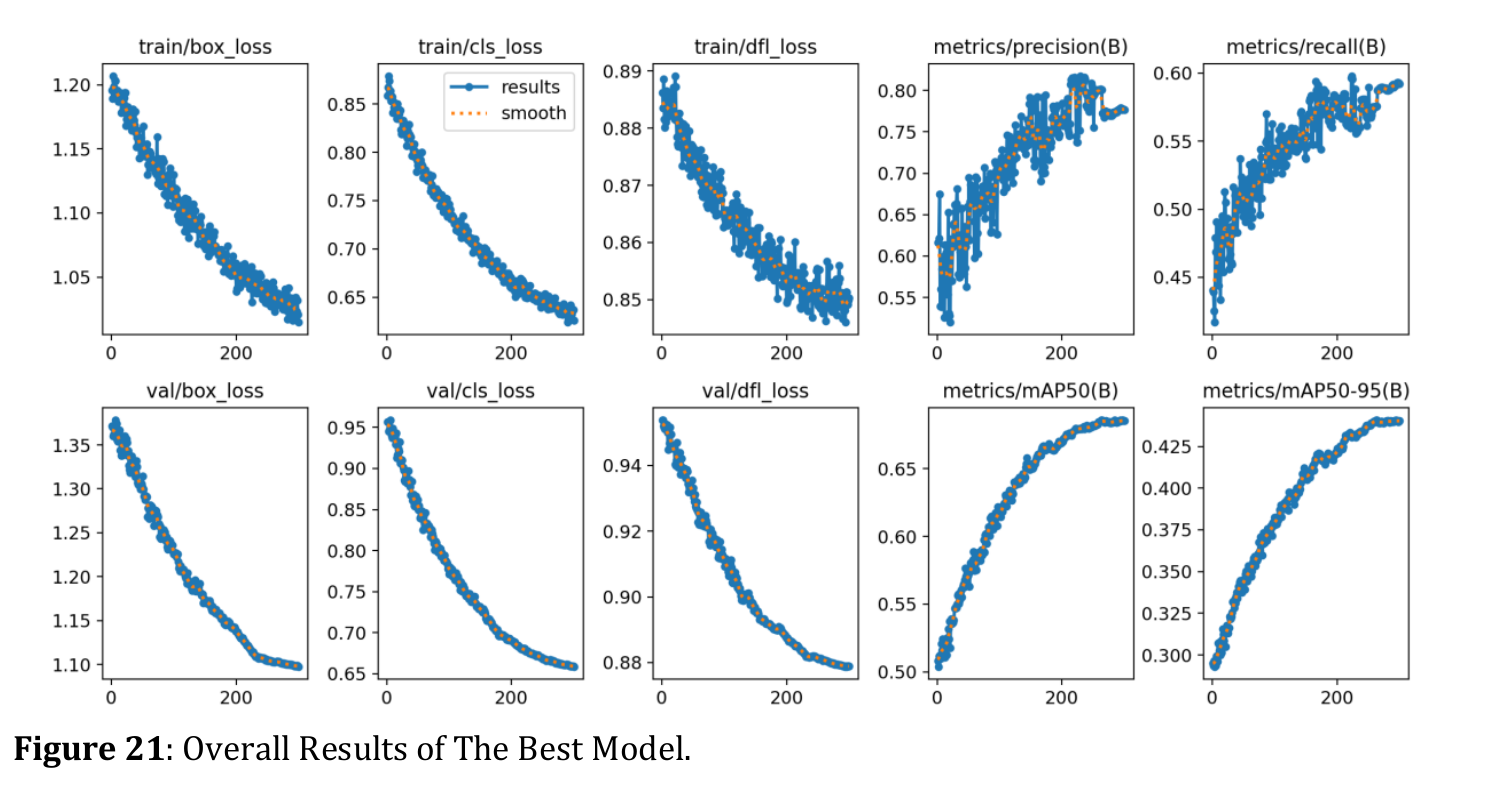
\includegraphics[width=0.9\textwidth]{v_5/paper_res.png}
            \subcaption{Modello dell'articolo}
            \label{fig:v5-4.1}
        \end{subfigure}
        \begin{subfigure}{.8\textwidth}
            \includegraphics[width=0.9\textwidth]{v_5/results.png}
            \subcaption{Nostro tentativo}
            \label{fig:v5-4.2}
        \end{subfigure}
        \caption{Comparazione tra l'andamento delle funzioni di errore durante il training
        del miglior modello dell'articolo e il nostro tentativo di replicare i risultati}
        \label{fig:v5-4}
    \end{figure}

In questo modo è stato possibile replicare i risultati e scoprire come le prestazioni
millantate nell'articolo siano viziate da un errore di impostazione dei sottoinsiemi
del dataset: gli autori hanno usato lo stesso set (probabilmente il train set)
sia per l'addestramento, che per la validazione che per il test. 
Il modello quindi non poteva raggiungere un alto valore di mAP50 
come indicato nell'articolo.
